\documentclass[10pt,journal,compsoc]{IEEEtran}
\usepackage[lmargin=2cm, rmargin=2cm, top=1.5cm, bottom=2.5cm]{geometry}
\usepackage{longtable,multirow,booktabs}
\usepackage{mathrsfs} % para formato de letra
\usepackage[spanish,es-tabla]{babel}
\usepackage[utf8]{inputenc}
\usepackage[usenames]{color}
\usepackage[dvipsnames]{xcolor}
\usepackage{amsmath}
\usepackage{amsfonts}
\usepackage{amssymb}
\usepackage{cancel}
\usepackage{graphicx}
\usepackage{tikz}
\usepackage{float}
\usepackage{fancyhdr}
\usepackage[hidelinks]{hyperref} 
\graphicspath{imagenes}
\title{\bfseries \huge {Comandos Git} }
\author{
	\IEEEauthorblockN{Ezequiel Remus} 
	{|} \IEEEauthorblockA{
		Email: ezequielremus@gmail.com}
}

\oddsidemargin=-1cm

\renewcommand{\footrulewidth}{0,01cm}
\begin{document}
%\pagestyle{myheadings}
%TITULO
%modificar el formato del titulo
\maketitle
\newpage
\tableofcontents
%\newpage
\pagestyle{fancy}

\section{Iniciales}
Tener en cuenta que el doble guión debe ser consecutivo. 

Todos los comandos git comienzan con la palabra \textbf{git}.
\begin{enumerate}
\item \underline{\textit{\color{Blue}{git - -version}}}:\\
 Para conocer la version de git que tenemos.
\\

\item \underline{\textit{\color{Blue}{git config - -global user.name $"nombreDeUsuario"$}}}:\\
Lo primero que tenes que hacer después de instalar \textbf{git} es establecer tu nombre de usuario (y también después de correo electronico). Este comando sirve para establecer tu nombre de usuario.
\\

\item \underline{\textit{\color{Blue}{git config - -global user.email $"TuCorreo"$}}}:\\
Lo primero que tenes que hacer después de instalar \textbf{git} es establecer tu nombre de usuario y correo electronico. Este comando sirve para establecer tu correo.
\\

\textbf{Para mas información sobre el comando \textit{config} utilizar el comando: \color{Blue}{git - -help config}}


\end{enumerate}
%\newpage
\section{Repositorios}
Hay varias formas para trabajar con repositorios, en particular la que explico primero sin haber creado el repositorio desde git y otra habiendo primero creado un repositorio (hablando de repos propios, ya voy a explicar como laburar con repos en grupo). Yo en particular les recomiendo la segunda que es mas rapida (para mi).

Empecemos con la primera:

Creamos una carpeta, abrimos git bash y corremos el comando \textit{\color{Blue}{git init}}. Este comando lo que hace es decirle a git que inicie el seguimiento de la carpeta sobre la cual corrimos el comando. El comando crea una carpeta oculta llamada \textit{.git} donde git almacena su base de datos. Para ver esta carpeta, corremos el comando \textit{ls -a} este muestra todos los directorios, incluso los ocultos.

Luego, dentro de nuestra carpeta repositorio creamos el archivo \textbf{README.md}. Este archivo es un archivo de texto markdown el cual se utiliza para realizar la descripción del repositorio e inclusive dar una idea de lo que esta documentado. Dentro de este pondremos el titulo del repositorio de la siguiente forma 
$$ \# Nombre del Repositorio $$
Este va a ser nuestro titulo del \textit{README.md}.

Luego de guardar el \textit{README.md} corremos el comando \textit{\color{Blue}{git status}} que nos sirve para conocer en que estado esta el proyecto. Los estados pueden ser 2, todo rojo o todo verde. Si esta en rojo, significa que el archivo esta modificado y no esta subido (todabia esta en el working directory) a la base de datos git, en cambio si esta en verde significa que lo subis al \textit{staging area}, que es el area de preparacion. Para mover el archivo de la zona de trabajo a el area de preparacion se utiliza el comando \textit{\color{Blue}{git add .}}, al pasarle el punto le decis que suba todos los modificados, si queres solo subir uno de esos archivos le pasas el nombre del archivo con su extencion.

Luego, para que el archivo forme parte de nuestro historial de proyecto es necesario hacer un \textbf{commit}, esto es subir el archivo al directorio de git. el comando completo es: \textit{\color{Blue}{git commit -m $"$Comentario que represente al commit$"$}}. (\textit{\color{Red}{No necesariamente se abre vim para agregar el mensaje, que es lo que dice en el tutorial, lo mas rapido es hacer el comando como se los pase yo sin tener que entrar a ningun editor de texto para escribir el mensaje}}). 

Si corremos \textit{\color{Blue}{git status}} despues de este paso, vamos a ver que nos dice que ya esta todo listo para subir. Para poder subirlo tenemos que asociar la carpeta a un \textbf{repositorido github} para luego realizar  un \textbf{push}.

Para hacer un repositorio, entramos a nuestra cuenta github y nos logeamos.
 \begin{figure}[H]
  \begin{center}
	 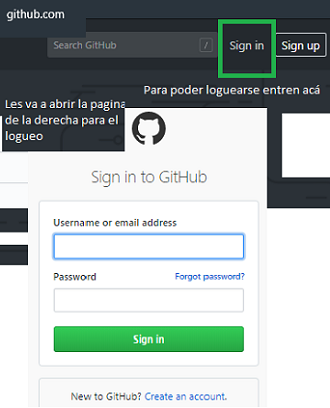
\includegraphics{figuras/logueo.png}
	 \centering
	 \renewcommand{\arraystretch}{1.3}
	 \caption{Pagina de github y logueo (aparecen en paginas diferentes)}
  \end{center}
\end{figure}

Despues del logueo van a la solapita con un signo de suma y apretan en \textbf{New Repository} 
 \begin{figure}[H]
  \begin{center}
	 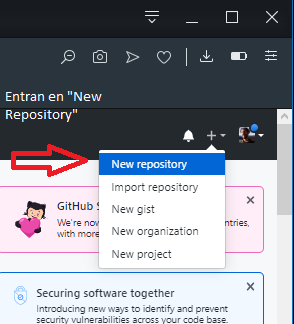
\includegraphics{figuras/repo.png}
	 \centering
	 \renewcommand{\arraystretch}{1.3}
	 \caption{Una vez logueados podemos crear un repo nuevo entrando a ese Boton}
  \end{center}
\end{figure}
Al entrar nos abre una ventana donde debemos tener en cuenta un par de cosas:

 Primero que nada, tenemos que ponerle un nombre si o si al repo (esto es poque sino no sabe a que corno apuntan los datos). 
 
 Por otra parte, \textit{yo prefiero en particular ahorrarme los pasos anteriores y crear primero el repositorio} con el \textit{README.md} desde la pagina (estamos hablando ya de la otra forma de las que les hable), te ahorras un par de comandos y es basicamente lo mismo.
 
  Los pasos anteriores sirven cuando ya tenes algo hecho y queres subirlo a un repo que ya existe o queres hacer un seguimiento de lo que fuiste haciendo a travez de los commits sin subirlo a un repositorio, en nuestro caso queremos trabajar con repos, por lo que les recomiendo primero crear el repositorio, clonar este en su pc (eso ya se los digo, es sencillo), poner los archivos que quieran subir y correr los comandos que venimos viendo de reconocimiento de estado, add y commit para poder subirlo y hacer el push directamente. Esto lo digo para que no se tengan que romper la cabeza para entrelazar la carpeta que creamos con las ramas del repositorio (origin y master) mediante comandos.
  
\begin{figure}[H]
  \begin{center}
	 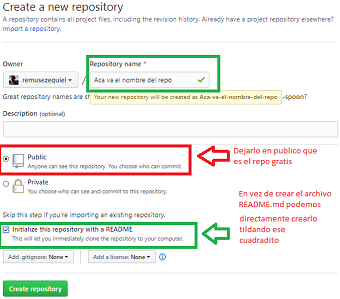
\includegraphics{figuras/crear.png}
	 \centering
	 \renewcommand{\arraystretch}{1.3}
	 \caption{Creando el repo}
  \end{center}
\end{figure}

Bueno, seguimos los pasos que aparecen en la \textit{Figura 3} y listo, ponemos \textbf{create repository} y se crea el repositorio. Yo cree uno para poner este pdf y despues voy a usarlo para poner apuntes, les dejo el link a este repositorio en las referencias por si lo quieren clonar cuando suba mas cosas y sino para que sepan que tambien pueden clonar repositorios de otros sin modificarles nada a los demas y asi poder leer las cosas de un repoistorio $x$ que les interese de una forma mas comodo.

\newpage
Bueno, siguiendo con esto de los repositorios, una ves creado el repositorio nos manda a la pagina del repo, que van a ver algo como esto:
\begin{figure}[H]
  \begin{center}
	 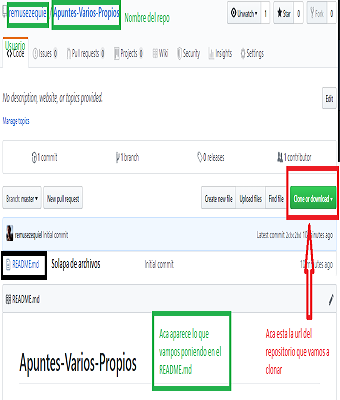
\includegraphics{figuras/repoNuevo.png}
	 \centering
	 \renewcommand{\arraystretch}{1.3}
	 \caption{Repo nuevo}
  \end{center}
\end{figure}
Ese es lo que se llama repositorio. Tenemos la parte de los archivos, donde ya de entrada vemos que aparece el archivo README.md, abajo de los archivos aparece lo que vamos escribiendo dentro del README (Si quieren no les ponen nada) este archivo es una guia sobre el repositorio, un resumen de lo que hay o muchas veces te explican como se usan o como se instalan los repositorios. Por ejemplo, estube viendo que el manejador de paquetes de Haskell \textit{Cabal} tiene su repositorio de github (dejo el link en referencias).
 
Ahora, para trabajar con este repositorio, tenemos que clonarlo en nuesto escritorio. Para eso, abrimos la terminal desde nuestro escritorio. tenemos que tener en cuenta, que si instalamos git en linux abrimos una terminal comun y nos corremos al Escritorio y ya esta, en windows, si siguieron los pasos del tutorial que puse en referencias para instalarlo e instalaron esa terminal que dice el pibe seria asi:

 \begin{figure}[H]
  \begin{center}
	 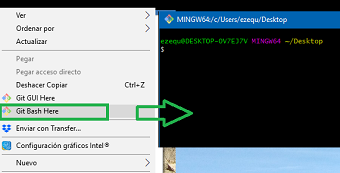
\includegraphics{figuras/consola.png}
	 \centering
	 \renewcommand{\arraystretch}{1.3}
	 \caption{Terminal desde windows}
  \end{center}
\end{figure}

Sino, si trabajan en linux y instalaron git con el comando \textit{\color{Green}{sudo apt-get install git}} abren una terminal de linux y corren los mismos comandos que voy a poner ahora, solo que clonan el repositorio que quieran clonar. En este caso, voy a clonar el repo que hice para este apunte. Para clonar el repositorio se utiliza el comando \textit{\color{Blue}{git clone urlDelRepositorio}}. El url lo sacan de la solapa \textbf{clone Repository} que esta en el repositorio, lo copian y lo pegan despues del comando git clone. Verifiquen que esten parados sobre el escritorio, sino se los va a clonar en otra ruta.

\begin{figure}[H]
  \begin{center}
	 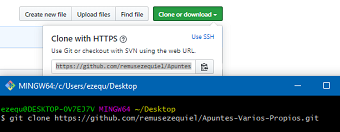
\includegraphics{figuras/clone.png}
	 \centering
	 \renewcommand{\arraystretch}{1.3}
	 \caption{Clonando el repositorio en el escritorio}
  \end{center}
\end{figure}

Vamos a ver que nos clona la carpeta en el escritorio con el nombre del repo. Abrimos la carpeta y vemos que el contenido es el mismo mas la carpeta oculta \textit{.git} de la que hablamos antes.

\begin{figure}[H]
  \begin{center}
	 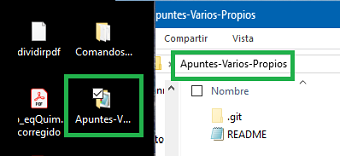
\includegraphics{figuras/carpeta.png}
	 \centering
	 \renewcommand{\arraystretch}{1.3}
	 \caption{Clonando el repositorio en el escritorio}
  \end{center}
\end{figure}

Ahora, lo que voy a hacer es poner la carpeta donde esta este pdf en el repositorio y voy a seguir los pasos de arriba:
\begin{figure}[H]
  \begin{center}
	 \includegraphics{figuras/Copio.png}
	 \centering
	 \renewcommand{\arraystretch}{1.3}
	 \caption{Pongo mi proyecto en el repo}
  \end{center}
\end{figure}
Ahora, abro una terminal sobre el repositorio o me corro adentre del repositorio, pero asegurense de estar dentro de la carpeta del repositorio y corro \textit{git status}.
\begin{figure}[H]
  \begin{center}
	 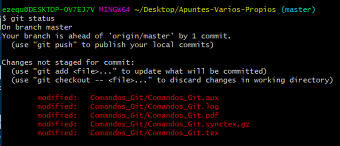
\includegraphics{figuras/StatusUno.png}
	 \centering
	 \renewcommand{\arraystretch}{1.3}
	 \caption{Realizo un status}
  \end{center}
\end{figure}
Como vemos, esta en rojo y nos dice $"$a estas cosas les podes hacer el add . $"$. Hacemos el \textit{add .} y corremos git status denuevo.
\begin{figure}[H]
  \begin{center}
	 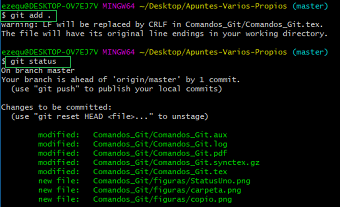
\includegraphics{figuras/add.png}
	 \centering
	 \renewcommand{\arraystretch}{1.3}
	 \caption{Realizo el add .}
  \end{center}
\end{figure}
\newpage
Ahora, hacemos el \textit{commit}:
\begin{figure}[H]
  \begin{center}
	 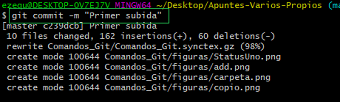
\includegraphics{figuras/commit.png}
	 \centering
	 \renewcommand{\arraystretch}{1.3}
	 \caption{Realizo el commit pasandole el comentario \textit{primer subida}}
  \end{center}
\end{figure}
Y ahora es la hora de hacer el push lo cual se hace con el comando \textit{\color{Blue}{git push origin master}}. Este comando lo voy a explicar mejor un poco mas adelante.
\begin{figure}[H]
  \begin{center}
	 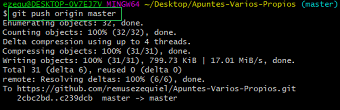
\includegraphics{figuras/push.png}
	 \centering
	 \renewcommand{\arraystretch}{1.3}
	 \caption{Realizo el push}
  \end{center}
\end{figure}

 Lo que es necesario entender hasta aca es que este comando lo sube a tu nube. Al ir a tu pagina en github, vas a ver que se renovo el repositorio de tu cuenta.
\begin{figure}[H]
  \begin{center}
	 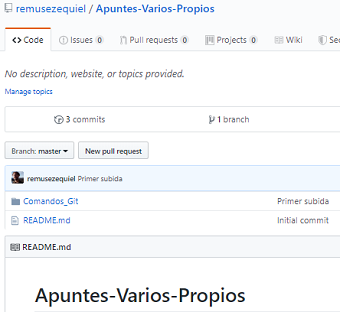
\includegraphics{figuras/repoPush.png}
	 \centering
	 \renewcommand{\arraystretch}{1.3}
	 \caption{Realizo el push vamos a la cuenta y vemos que se subieron las cosas (refresquen la pagina)}
  \end{center}
\end{figure} 


\section{Git Colavorativo}
\subsection{Introducción}
Supongamos que estás trabajando en un proyecto y queres agrgar una nueva funcionalidad. La forma correcta es creando un \textit{Branch} o  \textit{Rama} con el nombre de la nueva funcionalidad donde agregaremos nuestros cambios.

Por defecto, cuando creamos un repositorio tiene una rama llamada \textit{master} (Como buena practica, nada debe desarrollarse en master, pero eso es otro tema). Para esto estan las ramas para experimentar y hacer cambios.

Un Branch (Rama), es una copia del proyecto, bajo el control de versiones, de forma que los cambios realizados en esta rama no afecten al resto del proyecto y viceversa. En español esto dice que el \textit{Branching o Ramificación} es la manera de trabajar en diferentes versiones de un repositorio a la vez.

Un \textit{Fork} es una copia exacta de un repositorio; creando uno nuevo en tu cuenta de Github con una url diferente que podemos utilizar como un repositorio git cualquiera. Tendremos dos repositorios independientes y cada uno evoluciona de forma autonoma.

Un pull request es una petición que el propietario de un fork de un repositorio hace al propietario del repositorio original para que este último incorpore los commits que están en el fork.

\subsection{Pasos} 
 Los pasos a seguir para trabajar de forma colaborativa son:
 
 \begin{enumerate}
 \item Hacer \textit{fork} desde la interfaz de github del proyecto en el cual queremos colaborar.
 \item Clonamos el repositorio al que le hicimos \textit{fork}.
 \item Creamos una nueva rama para desarrollar nuestro aporte
 \item Realizamos los commits para describir las modificaciones u aportes.
 \item Se hace un push de las modificaciones en nuestra copia del repositorio
 \item Se pide un pull request desde la interfaz de github
 \end{enumerate}
\subsection{Comandos}
Vamos a tener que tener en claro que hace cada uno de estos comandos:
\begin{itemize}

\item \textit{\color{Blue}{git branch nombreDeLaRama}}: Crea la rama llamada nombreDeLaRama

\item \textit{\color{Blue}{git branch}}: Enlista todas las ramas en el repositorio actual.

\item \textit{\color{Blue}{git branch -d nombreDeLaRama}}: Elimina la rama especificada

\item \textit{\color{Blue}{git checkout nombreDeLaRama}}: cambia a la rama especificada

\item \textit{\color{Blue}{git remote -v}}

\item \textit{\color{Blue}{git remote add nombreQueVaATenerElRemoto url}}

\item \textit{\color{Blue}{git remote rename old new}}

\item \textit{\color{Brown}{git log --online}}
\end{itemize}

\subsection{Ahora a trabajar de verdad} 
Veamos como podemos aportar a un repositorio ya existente.

Imaginense que en mi cuenta tengo un repositorio en el cual vamos a trabajar los tres. Como el repositorio original, es decir el que tiene la rama master, es mio ustedes tienen que hacer la copia de mi repositorio en el suyo, esto se hace mediante el \textit{fork}. Supongamos que el repositorio al que le tienen que hacer fork es el repositorio con url \url{https://github.com/remusezequiel/Haskell-Algebra1}, ustedes tienen que entrar al repo y darle al fork.
\begin{figure}[H]
  \begin{center}
	 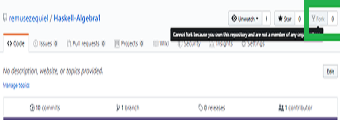
\includegraphics{figuras/fork.png}
	 \centering
	 \renewcommand{\arraystretch}{1.3}
	 \caption{Boton del fork (disculpen la calidad horrenda de imagen)}
  \end{center}
\end{figure} 
Al apretar ahi se genera en su cuenta una copia de mi repositorio (Si no me equivoco es una especie de puntero, pero desconosco como se enlaza a nivel programación). Ahora pueden trabajar con una copia de mi repositorio como si fuera de ustedes, y si lo modifican no van a modificar mi repositorio directamente. Para hacer que las modificaciones que hagan aparescan en mi repositorio basicamente yo tengo que aceptar sus cambios, porque el repo original es mio. Esto se hace para que justamente, si vos queres sacarle info a un desconosido porque te sirve o queres aprender de su codigo y modificarlo a tu gusto no modifiques directamente sus cosas, solo se puede modificar si el administrador te lo permite. El hace la copia del repo, pero no lo actualiza todo el tiempo a menos que vos lo actualizes cuando te convenga. 

Ya podemos clonar nuestro repositorio fork de la misma forma que lo hicimos en la sección 2.

Por defecto el al clonarlo el comando \textit{clone} crea por defecto el remoto \textit{origin} que apunta al fork que realizaste, es decir a tu repositorio. Fijense, corran el comando \textit{\color{Blue}{git remote -v}}, este les va a tirar algo parecido a esto:
\begin{figure}[H]
  \begin{center}
	 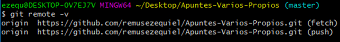
\includegraphics{figuras/gitRemote.png}
	 \centering
	 \renewcommand{\arraystretch}{1.3}
  \end{center}
\end{figure} 
Nos interesa mantener un enlace entre el repositorio original y con el fork, por lo tanto tenemos que renombrar el remoto que apunta al repositorio propio, para hacer esto tenemos que usar el comando \textit{\color{Blue}{git remote rename old new}}, donde \textit{old} representa el nombre actual del remoto (es decir origin) y \textit{new} es el nombre que queres ponerle vos al remoto, ejemplo: \textit{\color{Brown}{git remote rename origin papasConCheddar}}, en este caso cambiamos el nombre del remoto pasando de llamarse origin a papasConCheddar. Vean corran de nuevo el comando \textit{\color{Blue}{git remote -v}} y van a ver que en donde antes decia origin dice papasConCheddar.

Una vez hecho este paso tenemos que configurar el repositorio original, es decir el del tipo que esta administrando, para esto vamos al repositorio original en github y copiamos la url que usamos para clonar los repositorios, la del boton verde que dice clone or download. Una vez copiada la url, volvemos a la terminal y corremos el comando \textit{\color{Blue}{git remote add nombreQueVaATenerElRemoto url}}, ejemplo: \textit{\color{Brown}{git remote add remusEzequiel \url{https://github.com/remusezequiel/Haskell-Algebra1.git}}}. En particular puede ser el nombre que se les haga mas comodo a ustedes.

 Luego de hacer esto ustedes van a tener su repositorio enlazado tanto con su repositorio como con el mio, pueden comprobarlo corriendo \textit{\color{Blue}{git remote -v}} (no les pongo fotos porque no llegue a hacer una cuenta random para poder hacer la ejemplificacion mas grafica)

Ahora, ya tenemos todo enlazado, asi que podemos empezar a trabajar modificando los archivos del repositorio. En particular, no se debe modificar las cosas estando parados en la rama \textit{master}, por lo que \textbf{tenemos que crear una nueva rama y pararnos sobre esta antes de empezar a hacer una modificacion}. Hay un comando que al mismo tiempo de crearte una rama te deja parado sobre esta, el comando es \textit{\color{Blue}{git checkout -b nombreDeLaNuevaRama}}, ejemplo: \textit{\color{Brown}{git checkout -b ramita}}. Listo creamos la rama \textit{ramita} y nos movimos a esta, es decir, pasamos de estar en master a estar en ramita. Ahora, podemos realizar los cambios en el proyecto. Una vez que terminamos de realizar los cambios seguimos los pasos para hacer un commit (status, add ., status, commit -m $"$comentario$"$). Antes de realizar otra cosa, corran el comando \textit{\color{Brown}{git log --online}}, este te enlista todos los commits, vas a ver que el primer commit que te aparece es el que le corresponde a tu ultimo commit y que aparece con \textit{HEAD} apuntando a \textit{ramita}. 

Llego la hora de solicitarle al administrador que incluya los cambios en el repositorio original. Primero, tenemos que enviar la rama local al repositorio que le hiciste el fork, para esto corremos \textit{\color{Brown}{git push remoto rama}}, es decir, en nuestro caso la rama es ramita, porque estamos parados sobre la rama y el remoto es papasConCheddar. Ahora, los cambios que se van a enviar corresponden a la rama en la que estamos ubicados al momento de correr el push, en este caso la rama local se llama ramita. Como le dijimos que los cambios los realice en esa rama, el remoto se va a encargar de crear dicha rama si es que no esta creada todavia. Ahora, si van a su repositorio van a ver que existen dos ramas \textit{master y ramita}. Al lado de la rama \textit{ramita} hay un boton que dice \textbf{New Pull Request}, con ese boton le pedimos al administrador que acepte los cambios sobre el repositorio original (es decir, el repo del admin). Nos va a mandar a una especie de editor de mensajes donde podemos comunicarle al administrador que cambios hiciste y demas, por defecto se llena con el comentario del commit que hiciste. Luego apretamos en el boton verde de abajo que dice \textbf{Create pull request}. 

Una vez hecho el \textit{pull}, el administrador va a ser notificado. Ustedes lo unico que tienen que hacer es esperar a que el administrador acepte los cambios. El administrador los acepta haciendo una cosa que le dicen \textit{mergear un pull request}, esto es crear un nuevo commit en el repo original. Una vez hecho el merge, github les va a mandar un mensaje diciendo que sus cambios fueron aceptados. Si van a su repositorio, van a la solapa de pull request y van a ver que en si todavia no esta aceptado  va a aparecer como \textit{open} y si esta aceptado aparece como \textit{Merged}. 

Luego, tengamos en cuenta que una vez que hagamos un fork y modifiquemos las cosas usando la rama ramita el repositorio nestro va a estar desactualizado respecto del repositorio original, por lo que tenemos que traer el nuevo historial del repositorio original a nuestro repositorio forkeado. Para esto
nos movemos a la rama master con el comando \textit{\color{Blue}{git checkout master}}. Como el proyecto esta apuntando a dos remotos. Ahora tenemos que hacer un pull de origin con el comando \textit{\color{Blue}{git pull origin master}}, esto trae todo el historial nuevo de la rama master del repositorio original a la rama en la que estamos ubicados (master), luego tenemos que enviar ese historial a tu fork esto se hace con el comando \textit{\color{Blue}{git push papasConCheddar master}}. Y listo, ya tenemos todo actualizado. Luego, para mantener actualizado el repositorio respecto de los cambios que realize el administrador corremos el comando \textit{\color{Blue}{git pull origin master}} para traer los cambios del repositorio del administrador y para subirlo a sus repositorios solo deben corres \textit{\color{Blue}{git push origin master}}

%%%%%%%%%%%%%%%%%%%%%%%%%%%%%%%%%%%%%%%%%%%%%%%%%%%%%%%%%%%%%%%%%
\newpage
\begin{thebibliography}{1}
%
\bibitem{IEEEhowto:kopka}
 \emph{StackOverflow}, 
 Link: \textcolor{Red}{\url{https://stackoverflow.com}}
%
\bibitem{IEEEhowto:kopka}
 \emph{Link a un cursito de git basico}, 
 
 Link: \textcolor{Red}{\url{https://www.youtube.com/watch?v=m4wh8GhzcYg&list=PLmUnyBCRHkvUPkrsseI1SmMtYgfc-f8Kn&index=3}}
 %
 %
\bibitem{IEEEhowto:kopka}
Cuenta propia de github \emph{}.

 Link: \textcolor{Red}{\url{https://github.com/remusezequiel?tab=repositories}}
% 
%
\bibitem{IEEEhowto:kopka}
Repositorio de github donde se encuentra el codigo de este proyecto  \emph{}.

 Link: \textcolor{Red}{\url{https://github.com/remusezequiel/Apuntes-Varios-Propios}}
% 
%
\bibitem{IEEEhowto:kopka}
Repositorio de github donde se encuentra el proyecto Cabal  \emph{}.

 Link: \textcolor{Red}{\url{https://github.com/haskell/cabal}}
% 
%
\bibitem{IEEEhowto:kopka}
Mas links  \emph{}.

 Link: \textcolor{Red}{\url{https://guides.github.com/activities/hello-world/?source=post_page-----62dea67aa2eb----------------------}}


 Link: \textcolor{Red}{\url{https://www.linuxito.com/programacion/890-como-mantener-tu-fork-sincronizado-con-upstream-en-git}}

 Link: \textcolor{Red}{\url{https://blog.muktek.com/git-colaborativo-fd8baafb8614}}
\end{thebibliography}




\end{document}